% !TeX root = ../main.tex

\chapter{图神经网络算法}

\section{图神经网络概述}

图神经网络(Graph Neural Network)是一种运行在图结构上的神经网络。
传统神经网络一般只能处理欧几里得结构数据(Euclidean Structure Data),如图像、视频、语音等。
而图数据是一种蕴含着丰富的元素间关系信息的非欧几里得结构数据(Non-Euclidean Structure Data),如知识图谱数据、蛋白质结构数据等。
一些重要操作如卷积能在图像上运算,却不能在不规则的图数据上运算。
针对图数据的图神经网络便应运而生,并在社交网络、推荐系统等领域大展身手,近年来对图神经网络算法的研究越来越受到学术界和工业界的关注。

对图神经网络的研究与卷积神经网络(Convolutional Neural Network)的发展密不可分,后者能够提取多尺度的空间局部特征并将其组合成具有高表达性的表示,而图神经网络本质上也是提取拓扑图的空间特征并进行聚集。
但区别在于,卷积神经网络按照特定的顺序对顶点的特征进行叠加,且不考虑顶点间的关系,而图中没有自然顺序,图神经网络在每个顶点分别传播,与输入顺序无关,一般用顶点邻居状态的加权和更新顶点的隐藏状态(hidden state)。

\section{图神经网络结构}

\subsection{图结构}
\begin{definition}
    图G可以通过顶点集合V和边集合E来描述。
    \begin{equation}
        G=(V,E)
    \end{equation}
\end{definition}

\begin{definition}
    邻接矩阵$A$用于表示顶点之间的相邻关系,取值如下
    \begin{equation}
    A_{ij}=\left\{ \begin{array}{lr}1, \quad (v_i,v_j)\in E\\0,\quad else \end{array}\right.
    \end{equation}
\end{definition}

\begin{definition}
    度矩阵$D$用于表示各顶点的度,取值如下
    \begin{equation}
        D_{ii}=\Sigma _jA_{ij}
    \end{equation}
\end{definition}

\begin{definition}
    定义拉普拉斯矩阵L
    \begin{equation}
        L=I_N-D^{-\frac{1}{2}}AD^{-\frac{1}{2}}
    \end{equation}
    $L$为半正定矩阵,可分解为$L=U\Lambda U^{T}$,$U$是$L$的特征向量矩阵,$\Lambda=\left(\begin{array}{ccc}
        \lambda_{0} & & \\
        & \ddots & \\
        & & \lambda_{n-1}
        \end{array}\right)$
\end{definition}

\subsection{原始图神经网络模型}

图神经网络的概念首先是由F. Scarselli等人于2009年提出的,为了解决根据图上部分已标记顶点预测未标记顶点的问题。
原始图神经网络模型主要由两个部分组成,传播(propagation)和输出(output)

\subsubsection{传播}
将各个顶点的包含邻居信息进行聚集,得到状态表示$h_v$,可用于生成输出
\begin{equation}
    h_v=f(x_v,x_{co[v]},h_{ne[v]},x_{ne[v]})
\end{equation}
其中,$x_v$表示顶点v的特征,$x_{co[v]}$表示顶点v邻边的特征,$h_{ne[v]}$表示顶点v邻居的状态,$x_{ne[v]}$表示顶点v邻居的特征

根据Banach不动点理论,并将上式改写为矩阵形式,得到迭代过程
\begin{equation}
    H^{t+1}=F(H^t,X)
\end{equation}
其中$X$为所有特征,$H^t$表示第t次迭代中所有顶点的状态

\subsubsection{输出}
对与定点分类问题,将最后一次迭代得到的稳定状态作为顶点状态$H$
\begin{equation}
    O=G(H,X_N)
\end{equation}
$X_N$为所有顶点特征,$G$可以解释为前馈全连接神经网络

\subsubsection{训练方法}
设训练集中顶点$i$对应的标签和输出结果分别为$l_i$和$o_i$,定义损失函数
\begin{equation}
    loss=\Sigma ^n_{i=1} (l_i-o_i)
\end{equation}
用梯度下降法确定函数$F$和$G$中的权值和偏差

\subsubsection{局限性}
首先,用不动点的方式来计算隐藏状态需要的迭代次数过多,效率较低。
其次,在迭代过程中使用相同的参数,而较普遍的做法是在不同的神经网络层使用不同的权值并一起训练,来作为分层特征提取的方法,这个问题在下文的图卷积网络算法中得到了解决。
另外,更新顶点的隐藏状态是一个时序的过程,可以使用GRU、LSTM之类的RNN核。

\section{图卷积网络算法}
卷积神经网络模型在图像识别、自然语言处理等方面取得了巨大成果,卷积的本质就是利用核函数来加权求和来实现特征提取。受此启发,在图结构上重新定义卷积运算的工作开始不断出现。

\subsection{基于图谱方法的卷积}

\begin{theorem}
    时域卷积定理
    \begin{equation}
        \mathcal{F}\left[f_{1}(t) * f_{2}(t)\right]=\mathcal{F}\left[f_{1}(t)\right] \odot \mathcal{F}\left[f_{2}(t)\right]
    \end{equation}
    $*$为卷积运算符,$\odot$为哈达马积,即矩阵中逐元素相乘
\end{theorem}

\begin{definition}
    将傅里叶变换推广到图上,可定义图上的傅里叶变换$\mathcal{F}$
    \begin{equation}
        \mathcal{F}[f]=U^Tf
    \end{equation}
    $U$为定义2.4中$L$的特征向量矩阵
\end{definition}

\begin{definition}
    由定义2.5,可定义图上的卷积变换
    \begin{equation}
        (f_1*f_2)_G=U\left(\begin{array}{ccc}
            \mathcal{F}[f_2(\lambda_0)] & & \\
            & \ddots & \\
            & & \mathcal{F}[f_2(\lambda_{n-1})]
            \end{array}\right)U^Tf_1=U\ \mathcal{F}[f_2(\Lambda)]\ U^Tf_1
    \end{equation}
    $*$为图卷积运算符
\end{definition}

\subsection{初代图卷积网络}
J. Bruna在2014年提出了第一代图卷积网络(Graph Convolutional Network),主要是将定义2.6中$\mathcal{F}[f_2(\Lambda)]$换成卷积核$diag(\theta_i)$

\subsubsection{初代模型}
\begin{definition}
    考虑特征$x \in R^n$与参数为$\theta_i\in R^n$的卷积核$g_\theta(\Lambda)=diag(\theta_i)$在傅里叶域的卷积
    \begin{equation}
        x_{next}=\sigma (g_\theta*x)=\sigma (U g_\theta(\Lambda) U^Tx)
    \end{equation}
    \begin{equation}
        g_\theta(\Lambda)=\left(\begin{array}{ccc}
        \theta_{0} & & \\
        & \ddots & \\
        & & \theta_{n-1}
        \end{array}\right)
    \end{equation}
\end{definition}

\subsubsection{局限性}
每次前向传播都要计算$U diag(\theta_i) U^T$三者乘积,对于大规模图来说代价较高,另外从L进行特征分解得到U的代价也较大

\subsection{用切比雪夫多项式作卷积核的图卷积网络}
将卷积核$g_\theta(\Lambda)$用Chebyshef多项式$T_k(y)=cos(k\ arccos(y))$逼近

有$g_\theta(\Lambda)\approx \Sigma_{k=0}^K\theta_kT_k(\tilde \Lambda)$

$\tilde \Lambda=\frac{2\Lambda}{\lambda_{max}}-I_N$,其中$\lambda_{max}$为拉普拉斯矩阵L最大的特征值

此时考虑卷积$g_\theta*x\approx \Sigma_{k=0}^K\theta_kT_k(\tilde L)x$,其中$\tilde L=\frac{2L}{\lambda_{max}}-I_N$

取$\lambda_{max}\approx2,K=1,\theta_0=-\theta_1=\theta$

$g_\theta*x=\theta(I_N+D^{-\frac{1}{2}}AD^{-\frac{1}{2}})x=\theta(\tilde{D}^{-1 / 2} \tilde{A} \tilde{D}^{-1 / 2})x$,其中$\tilde{A}=A+I_N$,$\tilde{D}=D+I_N$

\begin{definition}
    故对于输入$X\in R^{n\times m}$,经过参数$\Theta\in R^{m\times m'}$的卷积核后的输出如下
    \begin{equation}
        X_{out}=\sigma\left(\tilde{D}^{-1 / 2} \tilde{A} \tilde{D}^{-1 / 2} X \Theta\right)
    \end{equation}
\end{definition}

\subsection{图卷积网络算法流程}
与卷积神经网络类似,图卷积网络的一次前向传播也由各图卷积层堆叠而成。
下文首先介绍一层图卷积层所作的计算,再介绍层之间的堆叠方式。
算法的具体实现参考了图神经网络框架DGL源码。

\begin{figure}[htb]
    \centering
    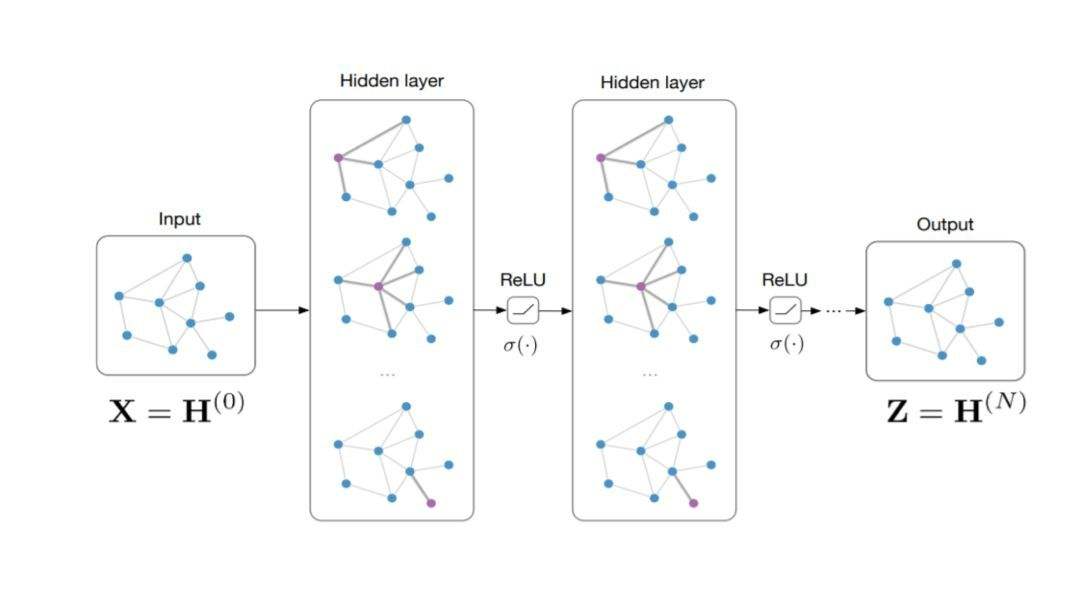
\includegraphics[width=\textwidth]{gcn.png}
    \caption{图卷积网络计算过程}
\end{figure}

\subsubsection{图卷积层}

\begin{definition}
    一次图卷积运算使用的公式如下
    \begin{equation}
        h_i^{(k+1)} = \sigma(b^{(k)} + \sum_{j\in\mathcal{N}(i)}\frac{1}{\sqrt{D_iD_j}} h_j^{(k)}W^{(k)})
    \end{equation}
    $h_i^{(k)}$表示第$k$层顶点$i$的隐藏状态,$\sigma$为激活函数,$b^{(k)}$表示第$k$层的偏差向量,$W^{(k)}$表示第$k$层的权值矩阵。
    $\mathcal{N}(i)$表示顶点$i$的所有邻居,$D_i$表示顶点$i$的度
\end{definition}

图卷积层的各参数如下
\begin{itemize}
    \item 输入参数。接收来自上一层的输出结果作为输入矩阵$H$,大小为顶点数$\times $输入特征长度($n\times m$)
    \item 固定参数。图中各顶点的度构成的向量$d$,大小为顶点数$\times 1$($n\times 1$)
    \item 待训练参数。权值矩阵$W$,大小为输入特征长度$\times$输出特征长度($m\times m'$)。偏差矩阵$B$,大小为$n\times$输出特征长度($1\times m'$)
\end{itemize}

运算过程如下。将向量$d$中各元素取$-\frac{1}{2}$次方后(若元素为0则变为1),按列填充成$n\times m$矩阵(每列均复制原始列向量),再与$H$和$W$矩阵乘的结果逐元素相乘得到$H'$,此矩阵可看作所有邻居的隐藏状态。
然后对图中每个顶点,将其邻居顶点在$H'$中对应的状态表示相加得到该顶点的聚集结果,按顶点顺序排列后得到新的状态矩阵$H_{new}$。
将向量$d$中各元素取$-\frac{1}{2}$次方后(若元素为0则变为1),按列填充成$n\times m'$矩阵,与$H_{new}$逐元素相乘后加上$B$,再经过激活函数$\sigma$得到输出结果。
至此,一层图卷积运算完成。

\subsubsection{层间堆叠}
一个完整的图卷积网络由许多上节所述的图卷积层堆叠而成,此处介绍一种堆叠方式。

\begin{itemize}
    \item 1层输入层。输入矩阵大小为顶点数$\times$输入特征长度,输出矩阵大小为顶点数$\times$隐藏特征长度,所取的激活函数为$ReLu$
    \item 若干层相同的隐藏层。输入和输出矩阵大小均为顶点数$\times$隐藏特征长度,在计算前将输入矩阵以0.5的概率做dropout,所取的激活函数为$ReLu$
    \item 1层输出层。输入矩阵大小为顶点数$\times$隐藏特征长度,输出矩阵大小为顶点数$\times$输出特征长度(一般为样本标签种类数),在计算前将输入矩阵以0.5的概率做dropout,无激活函数
\end{itemize}

\subsection{小结}
图卷积网络的基本思想是把图中顶点高维度的邻居信息聚集后用较低维的向量表示。
优点在于能利用整个图的信息,从而较好地表示出各顶点的状态。
缺点在于算法需要让图中所有顶点参与计算,当出现新增顶点时又需要重新从头开始训练,带来较大的计算开销。

\section{GraphSAGE算法}

\subsection{算法简介}
考虑到图卷积网络要求在训练过程中图的所有顶点均出现,这种直推式(transductive)的训练多用于固定的图,泛化能力较弱,无法对未出现过的顶点作出准确的预测。
本节介绍的GraphSAGE算法是一种归纳式(inductive)的训练,直接训练顶点的表示方法,能高效地利用顶点信息为未出现过的顶点生成嵌入(embedding)。

\begin{figure}[htb]
    \centering
    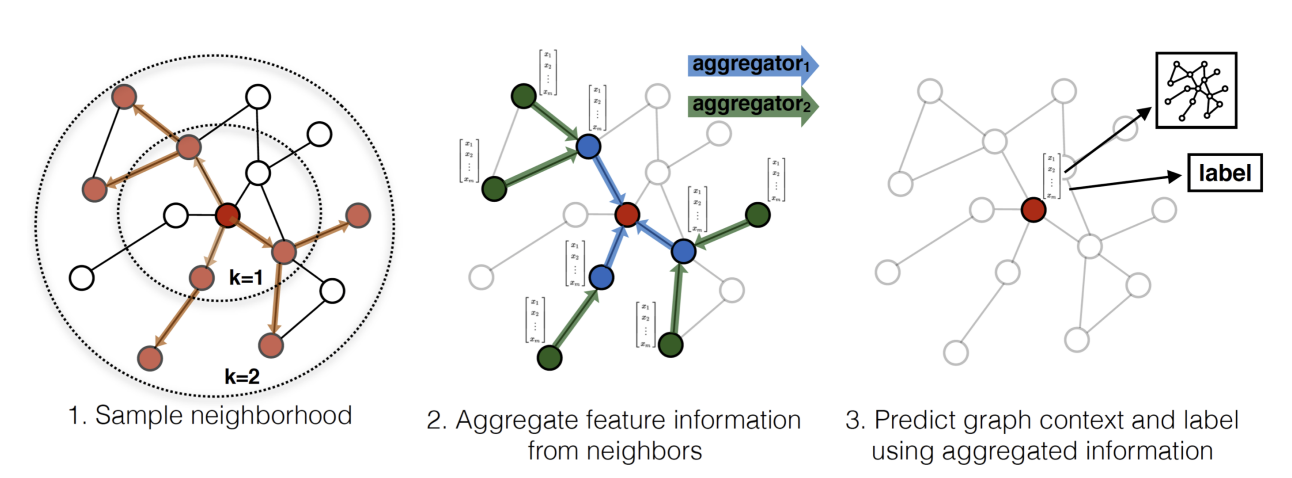
\includegraphics[width=\textwidth]{graphsage.png}
    \caption{GraphSAGE计算过程}
\end{figure}

GraphSAGE是Graph SAmple aggreGatE的缩写,即对图中各顶点的邻居进行采样和聚集,主要可以分为以下三个步骤
\begin{enumerate}
    \item 为每个顶点选取一定数量的邻居
    \item 根据聚集函数聚集邻居所蕴含的信息
    \item 得到图中各顶点的嵌入供下一层使用
\end{enumerate}

\subsection{算法流程}
与介绍图卷积网络算法流程的方式类似,讨论一次前向传播的流程。
本节先介绍对邻居进行采样的过程,再介绍一层SAGE卷积层所作的运算,以及层间的堆叠方式

\subsubsection{邻居采样}
此过程在数据预处理阶段进行,主要任务是为每层网络生成一个训练子图。

首先选择一组顶点加入终点集合,对该集合中每个顶点,分别为其选取固定数量的邻居顶点加入到起点集合中,由此构成的二分图即为一个训练子图。
再将起点集合作为下一轮迭代的终点集合重复上述过程,共进行$l$次($l$为网络层数)。最后将这批二分图逆序排列即为每层网络需要的训练子图。

\subsubsection{SAGE卷积层}
\begin{definition}
    一次SAGE卷积运算使用的公式如下
    \begin{equation}
        {h}_{\mathcal{N}(i)}^{(k)} = \operatorname{AGGREGATE}_{k}\left(\left\{{h}_{u}^{(k)}, \forall u \in \mathcal{N}(i)\right\}\right)
    \end{equation}
    \begin{equation}
        {h}_{i}^{(k+1)} = \sigma\left(b^{(k)} + \operatorname{CONCAT}\left({h}_{i}^{(k)}, {h}_{\mathcal{N}(i)}^{(k)}\right) \cdot {W}^{(k)}\right)
    \end{equation}
    $h^{(k)}_i$表示第$k$层顶点$i$的隐藏状态,$\sigma$为激活函数,$b^{(k)}$表示第$k$层的偏差向量,$W^{(k)}$表示第$k$层的权值矩阵。
    $\mathcal{N}(i)$表示顶点$i$的邻居采样结果,$\operatorname{AGGREGATE}$表示聚集函数,$\operatorname{CONCAT}$表示拼接函数。
\end{definition}

\paragraph{聚集函数}
图内部的顶点排列是无序的,所使用的聚集函数也应该是无序的。主要有以下三种聚集方式
\begin{itemize}
    \item 平均聚集。即对采样所得邻居的状态取平均值
    \item LSTM聚集。LSTM具有更强的表达能力,但由于不具有排列不变性,需要将采样所得邻居随机打乱后作为LSTM的输入
    \item 池化聚集。对顶点$i$所有采样所得邻居的状态先进行一次非线性变换后再做最大池化,即取每个特征方向上的最大值
\end{itemize}

\paragraph{拼接函数}
考虑矩阵形式的算法迭代。矩阵$H_{自身}$和$H_{邻居}$的大小都为顶点数$\times$输入特征长度,将两个矩阵按列拼接,得到大小为顶点数$\times$两倍输入特征长度的矩阵。
同时$W$的大小应为两倍特征长度$\times$输出特征长度。

\subsubsection{层间堆叠}
一个完整的SAGE卷积网络由许多上节所述的SAGE卷积层堆叠而成,此处介绍一种堆叠方式。

\begin{itemize}
    \item 1层输入层。输入矩阵大小为该层训练子图顶点数$\times$输入特征长度,输出矩阵大小为顶点数$\times$隐藏特征长度,所取聚集方式为平均聚集,激活函数为$ReLu$
    \item 若干层相同的隐藏层。输入和输出矩阵大小均为该层训练子图顶点数$\times$隐藏特征长度,在计算前将输入矩阵以0.5的概率做dropout,所取聚集方式为平均聚集,激活函数为$ReLu$
    \item 1层输出层。输入矩阵大小为该层训练子图顶点数$\times$隐藏特征长度,输出矩阵大小为顶点数$\times$输出特征长度(一般为样本标签种类数),在计算前将输入矩阵以0.5的概率做dropout,所取聚集方式为平均聚集,无激活函数
\end{itemize}

\subsection{小结}
GraphSAGE算法提出了聚集函数的概念,并且每次计算只使用一部分邻居,这种训练方式得到的模型具有较强的迁移能力,因而在新的类似的图上也能取得较好的效果,同时也较好地在准确率和计算代价间进行了折中。

\section{DiffPool算法}

\subsection{算法简介}
图上的机器学习问题一般包括顶点分类、链路预测和图分类。
对于前两类问题,可以直接将局部的顶点特征提取后进行聚集(相加或取最大值),比如图卷积网络算法和GraphSAGE算法中所做的。
但对于图分类问题,为了从顶点嵌入得到图的表示,如果直接简单相加或取最大值会忽略顶点间可能存在的层次关系。
据此,DiffPool算法提出了一个多层次的图神经网络模型,在每一层中不仅对顶点特征进行抽取,而且会把图结构重新聚合成一个更粗粒度的图以供下一层使用,这一步可以类比卷积神经网络中的池化层。
经过多层的信息抽取,最后将得到可以用于图分类的一个顶点的向量。

\begin{figure}[htb]
    \centering
    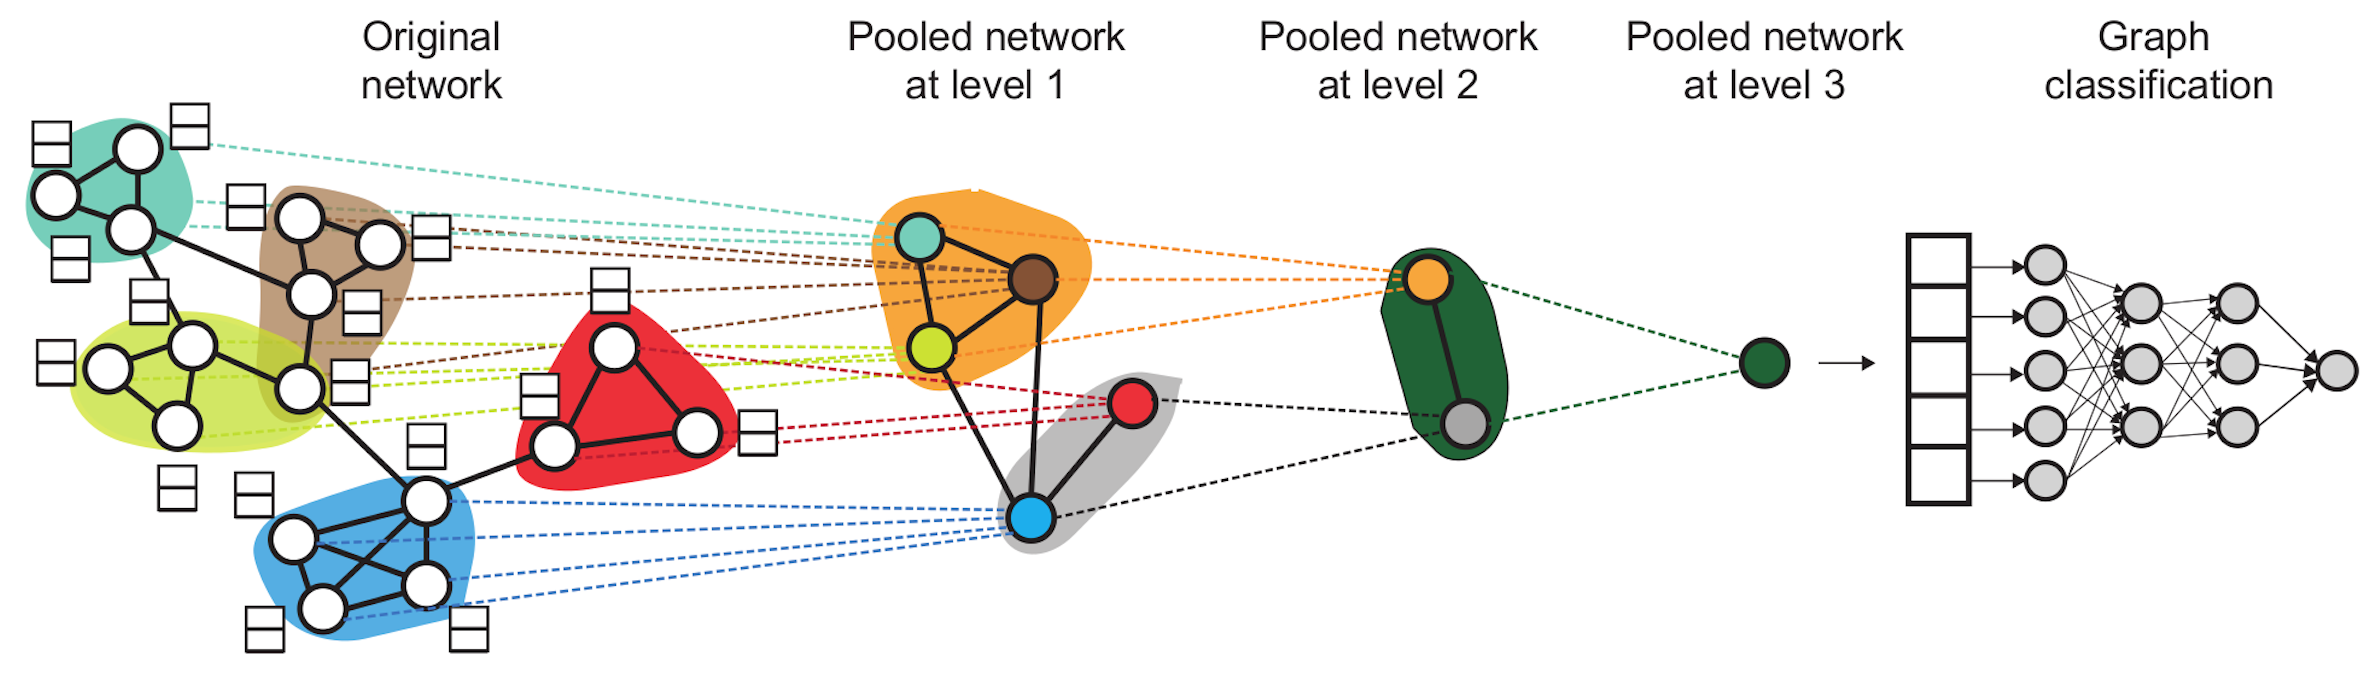
\includegraphics[width=\textwidth]{diffpool.png}
    \caption{DiffPool计算过程}
\end{figure}

\subsection{算法流程}
与介绍图卷积网络和GraphSAGE算法流程的方式类似,讨论一次前向传播的流程。
本节先讨论一层DiffPool层所做的运算,再介绍层间的堆叠方式。

\subsubsection{DiffPool层}
\begin{definition}
    一层运算涉及的公式如下
    \begin{equation}
        Z^{(l)}=\mathrm{GNN}_{l, \mathrm{embed}}\left(A^{(l)}, X^{(l)}\right) 
    \end{equation}
    \begin{equation}
        S^{(l)}=\operatorname{softmax}\left(\mathrm{GNN}_{l, \mathrm{pool}}\left(A^{(l)}, X^{(l)}\right)\right)
    \end{equation}
    \begin{equation}
        X^{(l+1)} =S^{(l)^{T}} Z^{(l)} \in \mathbb{R}^{n_{l+1} \times d}
    \end{equation}
    \begin{equation}
        A^{(l+1)} =S^{(l)^{T}} A^{(l)} S^{(l)} \in \mathbb{R}^{n_{l+1} \times n_{l+1}}
    \end{equation}
    $A^{(l)}$表示第$l$层所用图的邻接矩阵,$X^{(l)}$表示第$l$层所有顶点的特征,$\mathrm{GNN}$可以使用上两节中的图卷积网络或GraphSAGE。
    输入参数为$A^{(l)}$和$X^{(l)}$,输出参数为$A^{(l+1)}$和$X^{(l+1)}$
\end{definition}

一层运算使用两个参数不同的图神经网络模型,式(2.18)中的模型用于抽取特征得到$Z$,式(2.19)中的模型则用于生成分配矩阵$S$,它表示上层顶点特征以多少权值被分配到下层的哪些顶点中。
式(2.20)和(2.21)用于生成下一层所需的新的粗粒度图,且第$l+1$层顶点数$n_{l+1}$小于第$l$层顶点数$n_l$。
这种池化策略有较强的泛化能力,能在推理过程中适应不同的图结构。

\subsubsection{层间堆叠}
设总层数为$L$。

第一层输入为原始图的邻接矩阵$A^{(0)}$和特征矩阵$X^{(0)}$

中间第$l+1$层输入为第$l$层输出的邻接矩阵$A^{(l)}$和特征矩阵$X^{(l)}$

倒数第二层(即第$L-1$层)DiffPool时将$S^{(L-1)}$设为全1的向量,那么在第$L$层将得到一个整个图的嵌入表示,可用于后续的图分类任务。

\subsection{小结}
相比于图卷积网络和GraphSAGE算法,DiffPool算法的主要工作在于借鉴卷积神经网络的池化层,提出了一种对图结构进行池化的方法,并且模型是可微的,可以使用随机梯度下降来进行训练。
但缺点在于每次池化过程参数都不相同,需要分别训练,带来较大的计算成本和收敛难度。

\section{算法共性和算子介绍}
本节的主要目的是将前三节介绍的三个典型图神经网络算法中的相同部分提炼出来并形成算子,以便在后续的代码生成阶段尽可能的提高可重用性。

\subsection{算法共性}
根据前三节介绍的算法流程,图卷积网络可看作GraphSAGE算法的基础,而这二者又可视为DiffPool算法的基础。
图卷积网络算法主要包括聚集、组合两个过程,GraphSAGE算法比图卷积网络算法多了对邻居的采样过程和不同的聚集方式,DiffPool算法则比前两者多了池化的过程和一些额外的矩阵乘法。

\begin{figure}[htb]
    \centering
    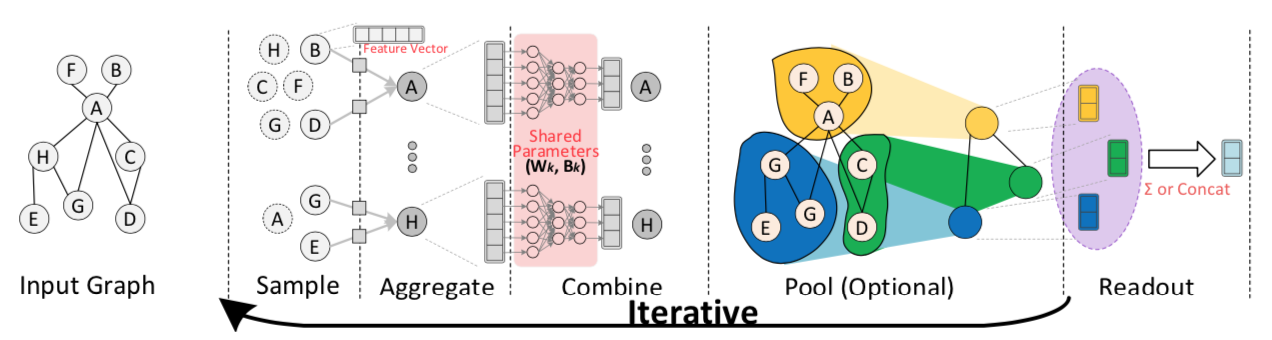
\includegraphics[width=\textwidth]{all.png}
    \caption{总体计算流程}
\end{figure}

\subsection{算子介绍}
根据上一小节所述,可以用以下四个算子实现三个典型算法:采样、聚集、组合、池化
\subsubsection{采样}
从每个顶点的邻居集合中选取包含固定数量顶点的子集,来作为该顶点新的邻居集合

\subsubsection{聚集}
将一个顶点邻居集合中所有顶点的特征向量按一定方式聚集成一个顶点向量,聚集方式有:相加、取平均值、经过非线性变换后取最大值等

\subsubsection{组合}
使用多层感知机(Multi-Layer Perceptron)将每个顶点的特征向量转变为其他长度的特征向量,但所有顶点共享相同的权值矩阵和偏差向量。
主要为矩阵运算和非线性激活。

\subsubsection{池化}
类似于卷积神经网络的池化层,通过分配矩阵(assignment matrix)降低顶点数,具体做法见第五节算法流程部分

\section{DGL图神经网络框架}
由于在之前讲述算法流程时参考了DGL框架的源代码,故此处对DGL做简单的介绍。
DGL(Deep Graph Library)是一个开源的图神经网络计算框架,由纽约大学和亚马逊公司主导开发,旨在为开发者提供一个基于现有深度学习框架(MXNet、PyTorch、TensorFlow)来进行图神经网络算法开发的平台。

作为一个易使用、高性能、可扩展的Python包,DGL的设计秉承以下三个原则:
\begin{itemize}
    \item 必须与主流的深度学习框架(MXNet、PyTorch、TensorFlow)无缝衔接,能方便地从传统的张量计算转变为图计算
    \item 应提供最少的API,降低用户的学习成本
    \item 保证上面两点的基础上,能高效透明地完成计算任务,并能方便地扩展到大规模图上
\end{itemize}

\begin{figure}[htb]
    \centering
    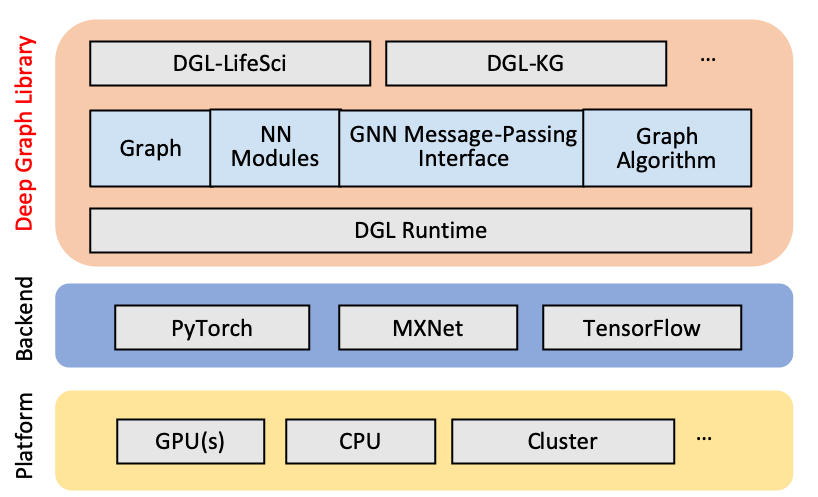
\includegraphics[width=\textwidth]{dgl.png}
    \caption{DGL整体架构图}
\end{figure}

从图2.5(DGL整体架构图)中可以看出,最上层是应用层,包括生命科学、知识图谱等;第二层有DGL框架定义的图结构、神经网络模块、消息传递接口和一些图算法;
再下层是DGL的运行时库,这部分主要由C++实现,编译成链接库后供Python层调用;后端由深度学习框架(MXNet、PyTorch、TensorFlow)提供支持,可运行于CPU、GPU等硬件上。

下面介绍上节列出的算子在DGL中的实现方法。聚集邻居顶点特征的过程在DGL框架中大致分为发送和接收两步。发送阶段将图中所有边源点的特征向量加权后沿着边向终点发送,接受阶段对每个顶点将沿着其邻边传递来的数据根据设定的聚集方式进行聚集。
用户可以自定义消息传递函数和接受函数,具体实现参考DGL源代码的update\_all函数。
组合过程和池化过程可以看成矩阵运算和非线性变换,主要由下层神经网络框架的线性层和激活函数实现。
采样过程暂无简单易用的API,此处不表。